\documentclass[12pt]{article}
\usepackage[margin=1in]{geometry} 
\usepackage{amsmath,amsthm,amssymb,amsfonts}
\usepackage{placeins}
\usepackage{mathtools, eucal}
\usepackage{color}
 

 
\begin{document}
 
%\renewcommand{\qedsymbol}{\filledbox}
%Good resources for looking up how to do stuff:
%Binary operators: http://www.access2science.com/latex/Binary.html
%General help: http://en.wikibooks.org/wiki/LaTeX/Mathematics
%Or just google stuff
 
\title{Homework 2 Solutions}
\author{Zheming Gao}
\maketitle


\section*{Problem 1}

Since there is an absolute value in the objective function and $x_3$ is unrestricted, we may divide the feasible domain into two parts: $x_3 \geqslant 0$ and $x_3 < 0$.

For $x_3 \geqslant 0$, $|x_3| = x_3$. Hence, we may construct a LP problem:

\begin{equation*}
\begin{aligned}
\text{Manximize} \quad & 3x_1 - 2x_2 + 4 x_3 \\
\text{subject\  to} \quad & -x_1 + 2 x_2 \leqslant -5 \\
& 3 x_2 - x_3 \geqslant 6 \\
& x_1, x_2, x_3 \geqslant 0
\end{aligned}
\end{equation*}

Similarly, for $x_3 < 0$,$|x_3| = -x_3$, and we can also construct a LP problem:

\begin{equation*}
\begin{aligned}
\text{Manximize} \quad & 3x_1 - 2x_2 - 4 x_3 \\
\text{subject\  to} \quad & -x_1 + 2 x_2 \leqslant -5 \\
& 3 x_2 - x_3 \geqslant 6 \\
& x_1, x_2 \geqslant 0, x_3 \leqslant 0.
\end{aligned}
\end{equation*}

Then convert those two LP problems above into standard forms:

\begin{equation}\label{L1}
\begin{aligned}
\text{Minimize} \quad & -3x_1 + 2x_2 - 4 x_3 \\
\text{subject\  to} \quad & -x_1 + 2 x_2 + \xi_1 = -5 \\
& 3 x_2 - x_3 - \xi_2 = 6 \\
& x_1, x_2, x_3, \xi_1, \xi_2 \geqslant 0
\end{aligned}
\end{equation}

and 

\begin{equation}\label{L2}
\begin{aligned}
\text{Minimize} \quad & -3x_1 + 2x_2 - 4 x_3 \\
\text{subject\  to} \quad & -x_1 + 2 x_2 + \xi_1 = -5 \\
& 3 x_2 + x_3 - \xi_2 = 6 \\
& x_1, x_2, x_3, \xi_1, \xi_2 \geqslant 0
\end{aligned}
\end{equation}

Take the optimal solution as the one that solves (\ref{L1}) or (\ref{L2}) with a smaller optimal value.



\section*{Problem 2.1}

Solutions: 

\begin{enumerate}
\item
We need to show that if the feasible domain is bounded, then the LP problem has a bounded optimal value.

\begin{proof}

Consider the standard form of a LP problem.

\begin{equation*}
\begin{aligned}
\text{Minimize} \quad & c^Tx \\
\text{subject\  to} \quad & Ax = b \\
 & x \geqslant 0
\end{aligned}
\end{equation*}

where $A \in \mathbb{R}^{m\times n}$, $x\in \mathbb{R}^n$, $b \in \mathbb{R}^m$.

Denote its feasible domain as $P := \{x \in \mathbb{R}^n | Ax = b, x \geqslant 0 \}$. If P is bounded, then $\exists M \geqslant 0$ such that $||x|| \leqslant M$ for all $x \in P$.

Recall Cauchy-Schwartz inequality, $\forall x, y \in \mathbb{R}^n$, 
$$
|x^Ty| \leqslant ||x||\cdot||y||
$$

Hence, we have 
$$
c^Tx \geqslant - ||c||\cdot ||x|| = ||c||(-||x||) \geqslant ||c||\cdot (-M).
$$

Since $c$ is a constant vector, $M$ exists as a constant, we know $c^Tx$ has a lower bound, which proves that the LP problem is bounded.

\end{proof}

\item

Next we give a counterexample to show that the opposite direction is not ture. 

Consider the following LP problem:

\begin{equation}\label{L2}
\begin{aligned}
\text{Minimize} \quad & 2x_1 + x_2 \\
\text{subject\  to} \quad & x_1 + x_2 \geqslant 1 \\
& x_1, x_2 \geqslant 0
\end{aligned}
\end{equation}

It is obvious that the feasible domain is not bounded but the problem is bounded.

\end{enumerate}


\section*{Problem 2.2}

\textbf{\color{red}ATTENTION: } The definitions of POLYHEDRON and POLYTOPE are on page 16, Chapter 2.

\begin{enumerate}
\item [(a)]
All of the claims are false. Counterexample is the unit plate ($S = \{(x, y) | x^2 + y^2 \leqslant 1\}$) on $\mathbb{R}^2$.

\item [(b)]
(i) is true. 
\begin{proof}

$\forall x, y \in S$, their affine combination is also in $S$. Hence, $\forall \alpha \in (0, 1)$, $\alpha x + (1-\alpha) y \in S$. Since it is the convex combination of $x$ and $y$, it proves the $S$ is convex.

\end{proof}

(ii), (iii) and (iv) are false. For example, let $S = \{(x, y) \in \mathbb{R}^2 | x + y = 1\}$. $S$ is a line on $\mathbb{R}^2$ but it doesn't satisfy the definition of cone. Also, it is obvious $S$ is not a polyhedron or polytope.

\item[(c)] 



\end{enumerate}


\section*{Problem 2.3}

\begin{proof}

To prove $H$ is affine, take $x, y$ from $H$ arbitrarily and we need to show the affine combination of $x$ and $y$ is also in $H$. This is true, since for any $\alpha_1, \alpha_2 \in \mathbb{R}$ that satisfy $\alpha_1 + \alpha_2  =1$, 

$$
a^T(\alpha_1 x + \alpha_2 y) = \alpha_1 a^T x + \alpha_2 a^T y = \alpha_1\beta + \alpha_2 \beta = \beta.
$$

which shows $\alpha_1 x + \alpha_2 y$ is in $H$.

For convexity, it follows from the fact that $H$ is affine because the convex combination of two points is a special case of their affine combination.

\end{proof}


\section*{Problem 2.4}

\begin{enumerate}
\item

\begin{proof}

We want to show $\forall x, y \in \cap_{i = 1}^ p C_i$, the convex combination of $x, y$ is also in it.

Since $x, y \in \cap_{i = 1}^ p C_i$, we know $x, y \in C_i$, $\forall i = 1,\dots, p$. with the fact that $C_i$ is convex, for any $\alpha \in (0, 1)$, $\alpha x + (1-\alpha) y \in C_i$ holds for each index $i$. Hence, $\alpha x + (1-\alpha) y \in \cap_{i=1} ^ p C_i$. 

The claim is then proved.

\end{proof}

\item
$\cup_{i=1}^p$ may not be convex. A counterexample is to let $C_1 = \{(x, y)| x = 0, y\in\mathbb{R}\}$, and $C_1 = \{(x, y)| y = 0, x\in\mathbb{R}\}$. It is clear that $C_1, C_2$ are convex and they are $x$ and $y$ axis in $\mathbb{R}^2$. However, $C_1\cup C_2$ is not convex. 

Let $a = (1, 0) \in C_2$, $b = (0, 1)\in C_1$. $a, b \in C_1\cup C_2$, but $\frac{1}{2} a + \frac{1}{2}b = (1/2, 1/2) \notin C_1\cup C_2$.

\end{enumerate}


\section*{Problem 2.5}

(It will be easy to use the results from the problems we just solved. But it is fine if you use other methods to prove this claim.)

\begin{proof}

Let $A \in \mathbb{R}^{m\times n}$ be $\begin{bmatrix}
a_1^T \\
\vdots \\
a_m^T
\end{bmatrix}
$, where $a_i^T$ is the ith row of $A$. 
and $b = [b_1, \cdots, b_m]^T$. Then the feasible domain $P$ is equivalent to 

$$
\cap_{i=1}^m \{ x\in\mathbb{R}^n | a_i^T x = b_i  \} \cap \{x\in\mathbb{R}^n | x \geqslant 0\}.
$$

Let $P_i : = \{ x\in\mathbb{R}^n | a_i^T x = b_i  \}$ and each $P_i$ is a hyperplane. Also, it is obvious that $\{x\in\mathbb{R}^n | x \geqslant 0\}$ is convex(use the definition and easy to prove). Use the results from 2.3 and 2.4, and we know that the $P_i$ is convex and intersection of convex sets is also convex. Hence, $P$ is convex.

\end{proof}

\section*{Problem 2.6}

\begin{proof}

Consider a LP problem in standard form. 

\begin{equation*}
\begin{aligned}
\text{Minimize} \quad & c^Tx \\
\text{subject\  to} \quad & Ax = b \\
 & x \geqslant 0
\end{aligned}
\end{equation*}

where $A \in \mathbb{R}^{m\times n}$, $x\in \mathbb{R}^n$, $b \in \mathbb{R}^m$.

Denote its feasible domain as $P := \{x \in \mathbb{R}^n | Ax = b, x \geqslant 0 \}$. Let the supporting hyperplane $H$ of feasible domain $P$ be the following,

$$
H: = \left\{  x\in\mathbb{R}^n| -c^Tx = \beta \right\}.
$$

and $\forall x\in P$, $-c^Tx \leqslant \beta$. since $H\cap P \neq \phi$, take any $x^* \in H\cap P$, we have $c^Tx^* =  -\beta$. Hence, $\forall x\in P$, $c^Tx \geqslant c^Tx^* = -\beta$, which proves that $x^*$ is an optimal solution to the LP problem.

\end{proof}

\section*{Problem 2.8}
From problem 2.7, the feasible region is 

\begin{figure}[htbp]
  \caption{Feasible region $P$.}
  \centering
    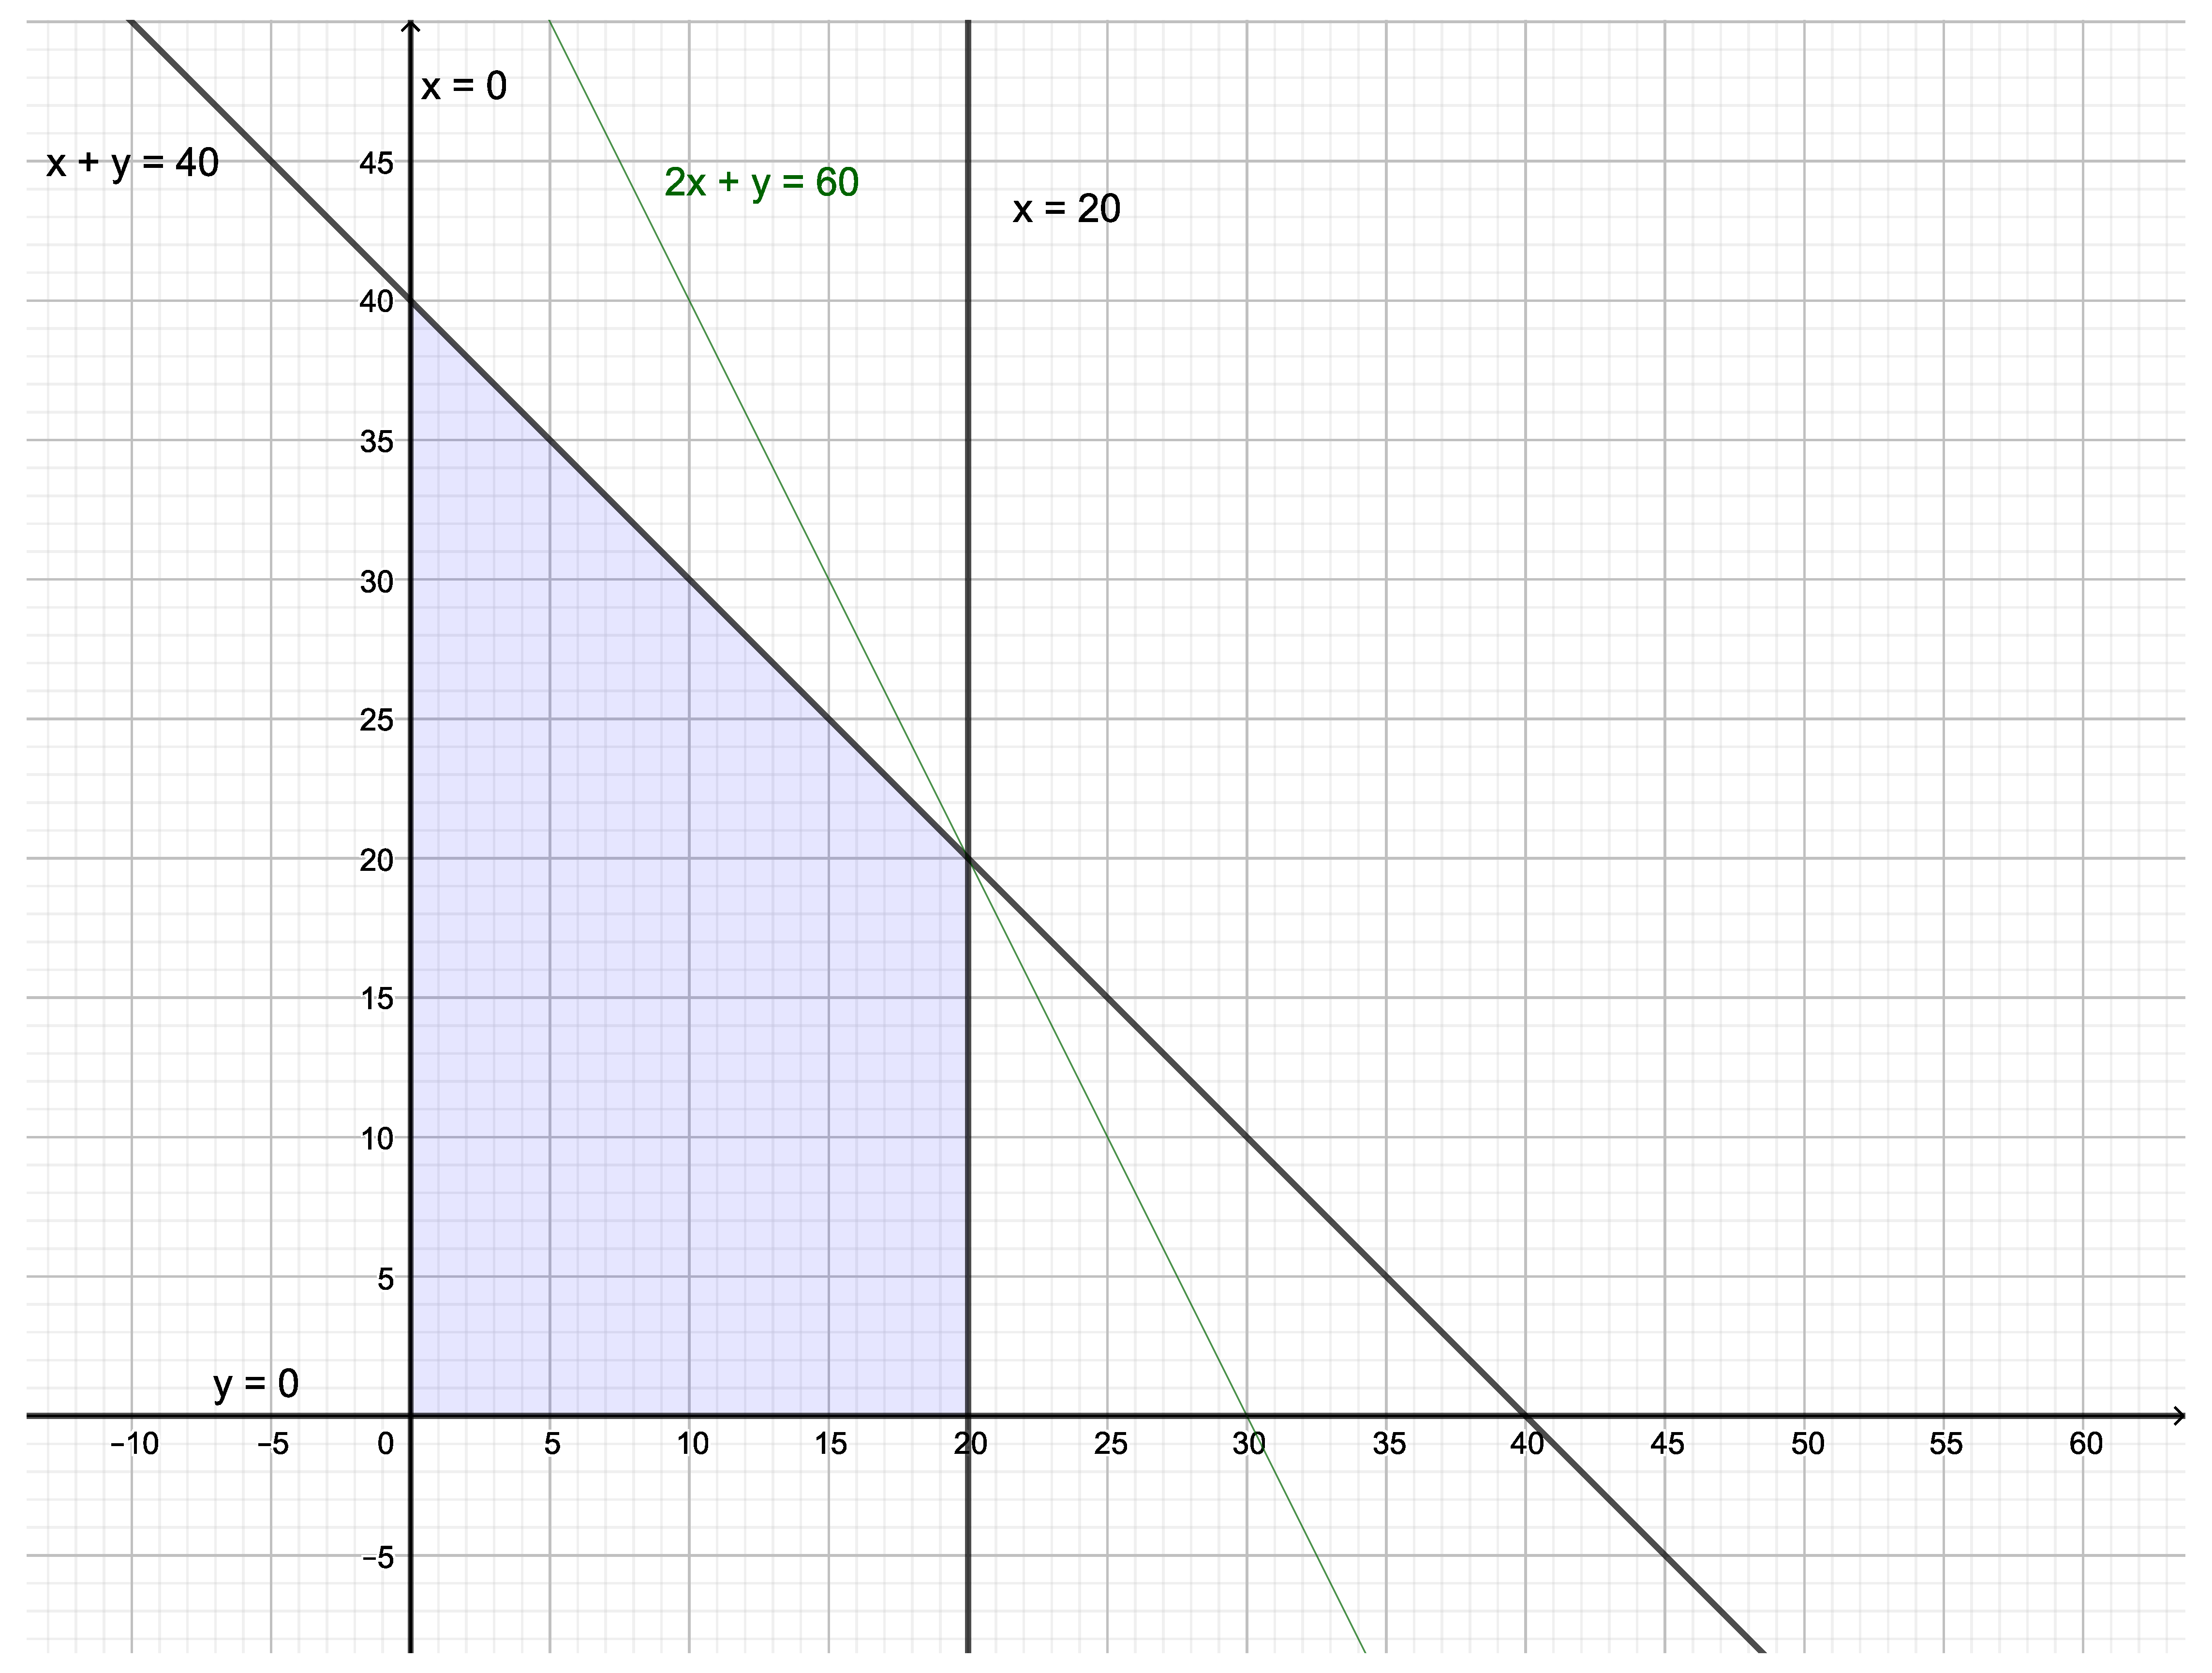
\includegraphics[width=0.5\textwidth]{2_8P.pdf}
\end{figure}

In our figures, $x$ is $x_1$ and $y$ is $x_2$. Using the graphic method and we get the results in following figures.

\begin{figure}[htbp]
  \caption{solution to (a)}
  \centering
    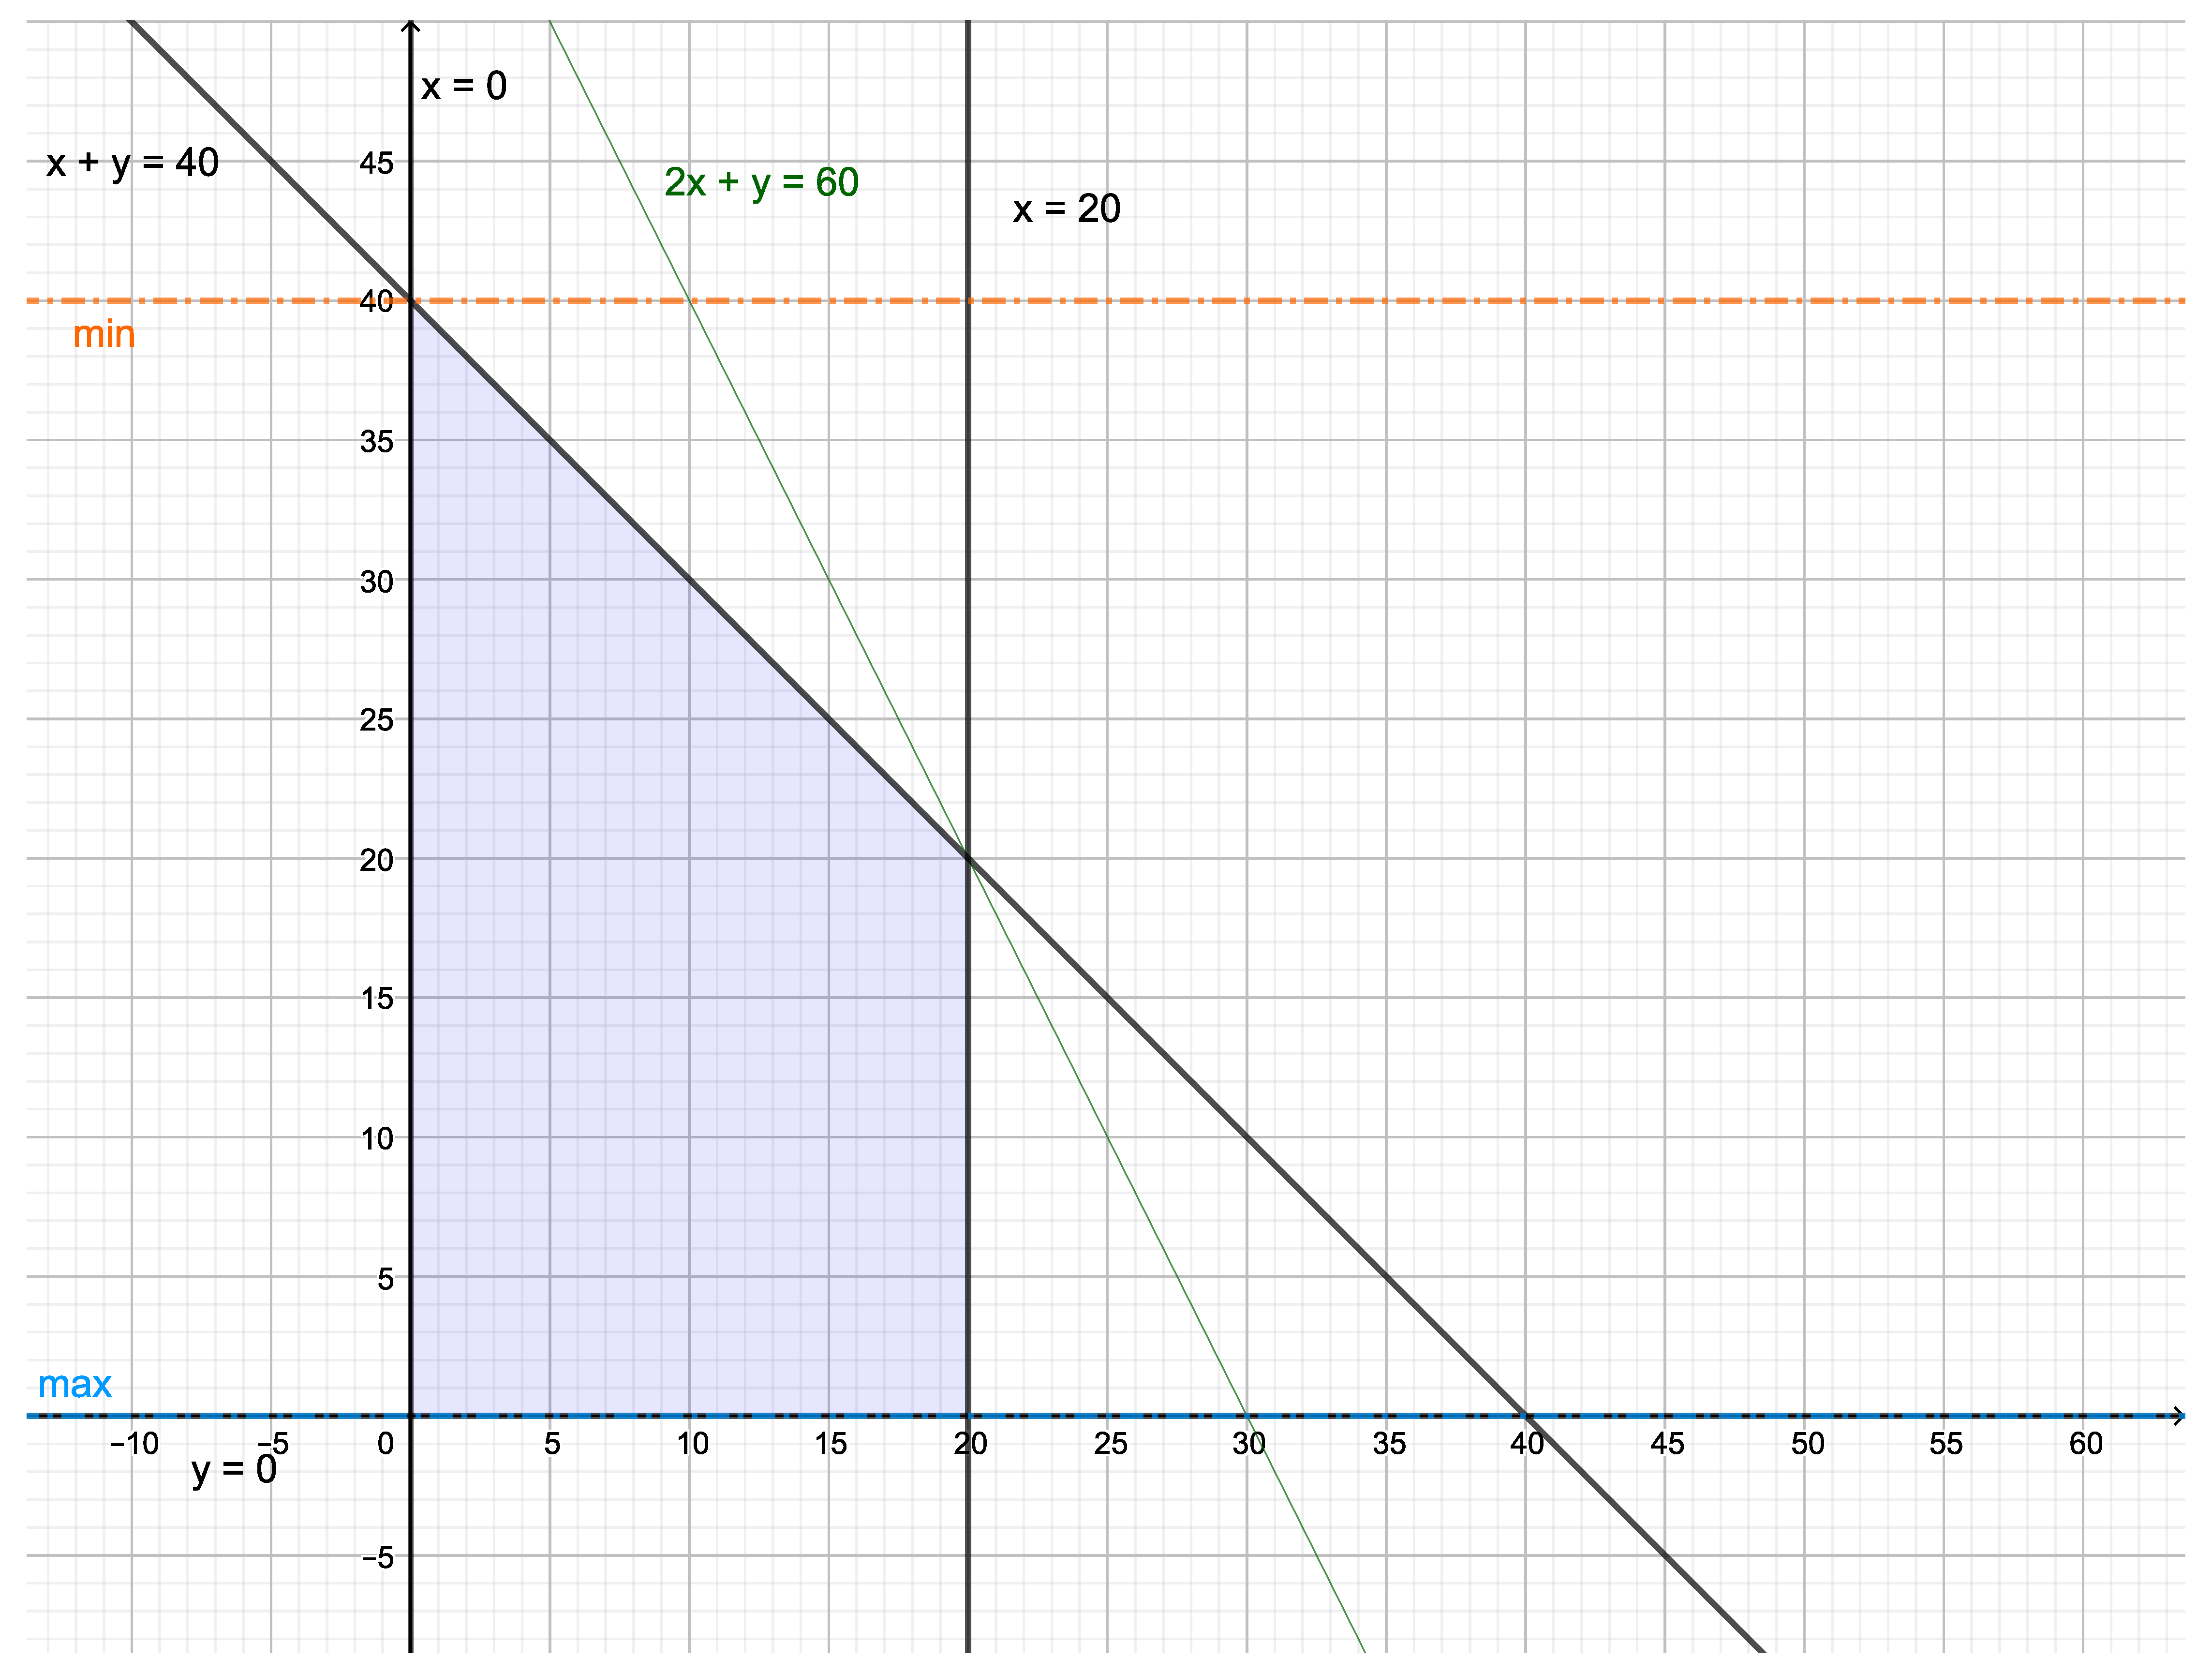
\includegraphics[width=0.5\textwidth]{2_8a.pdf}
\end{figure}

\begin{figure}[htbp]
  \caption{solution to (b)}
  \centering
    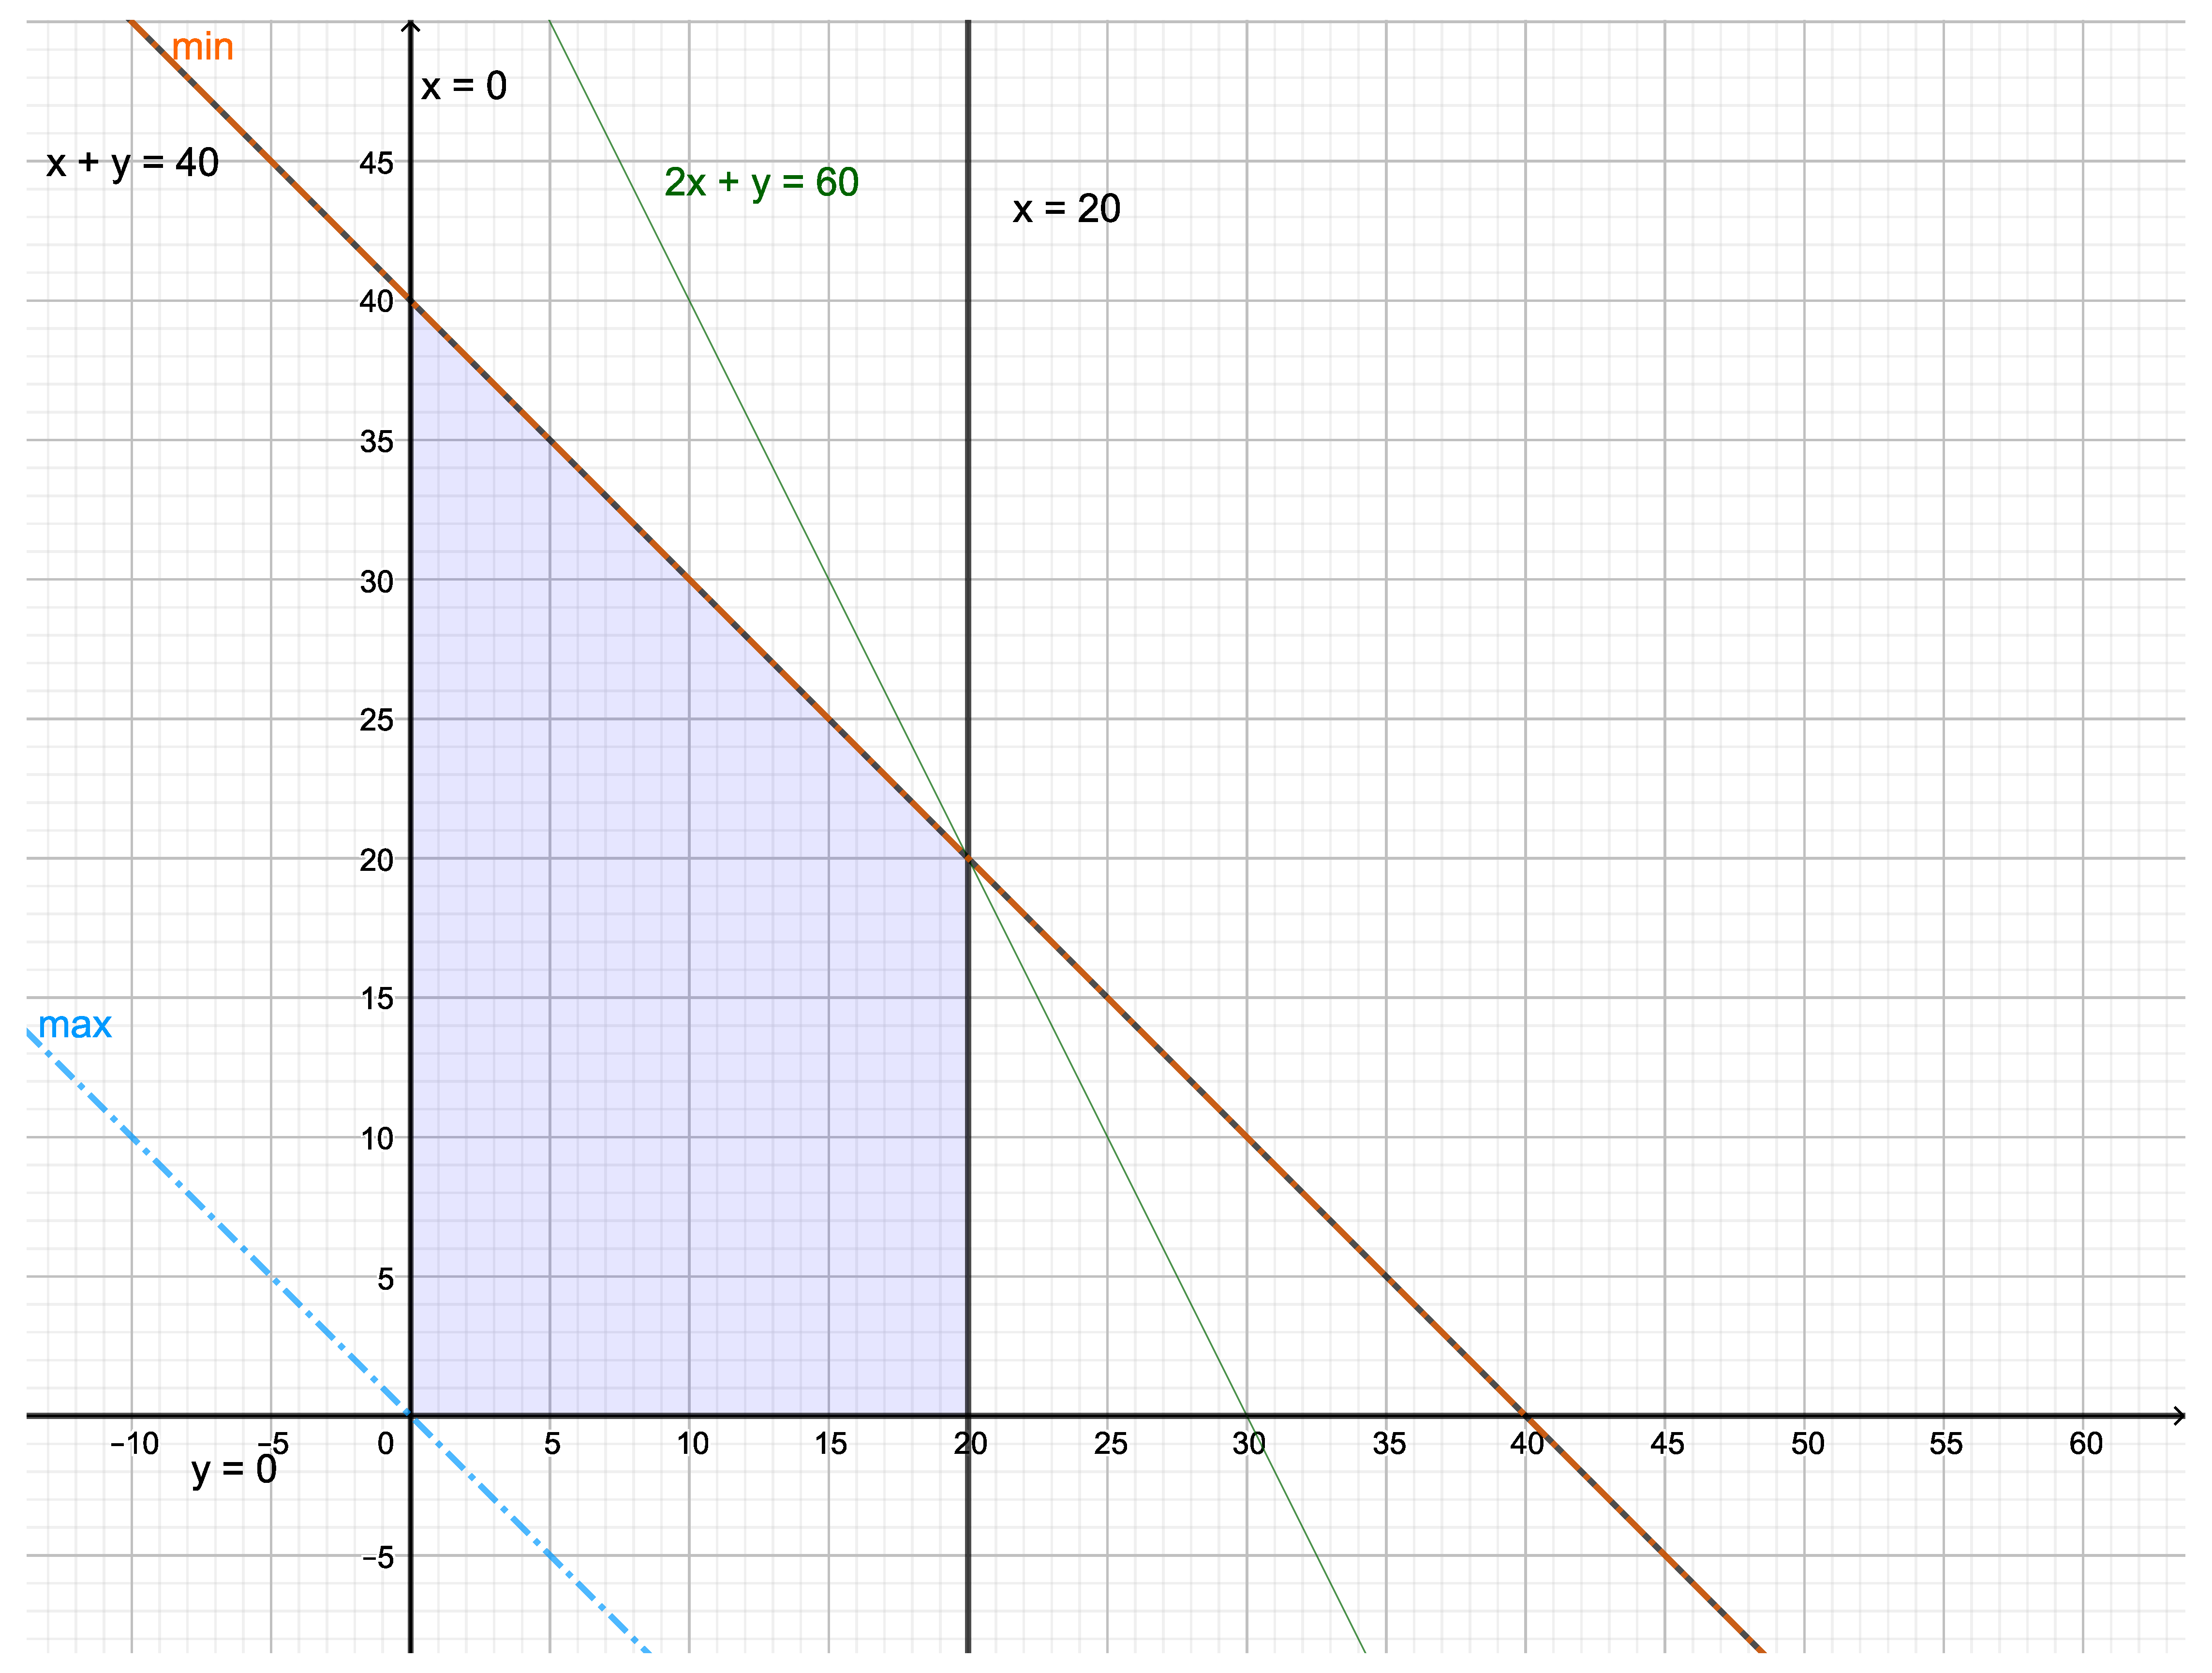
\includegraphics[width=0.5\textwidth]{2_8b.pdf}
\end{figure}
\begin{figure}[htbp]
  \caption{solution to (c)}
  \centering
    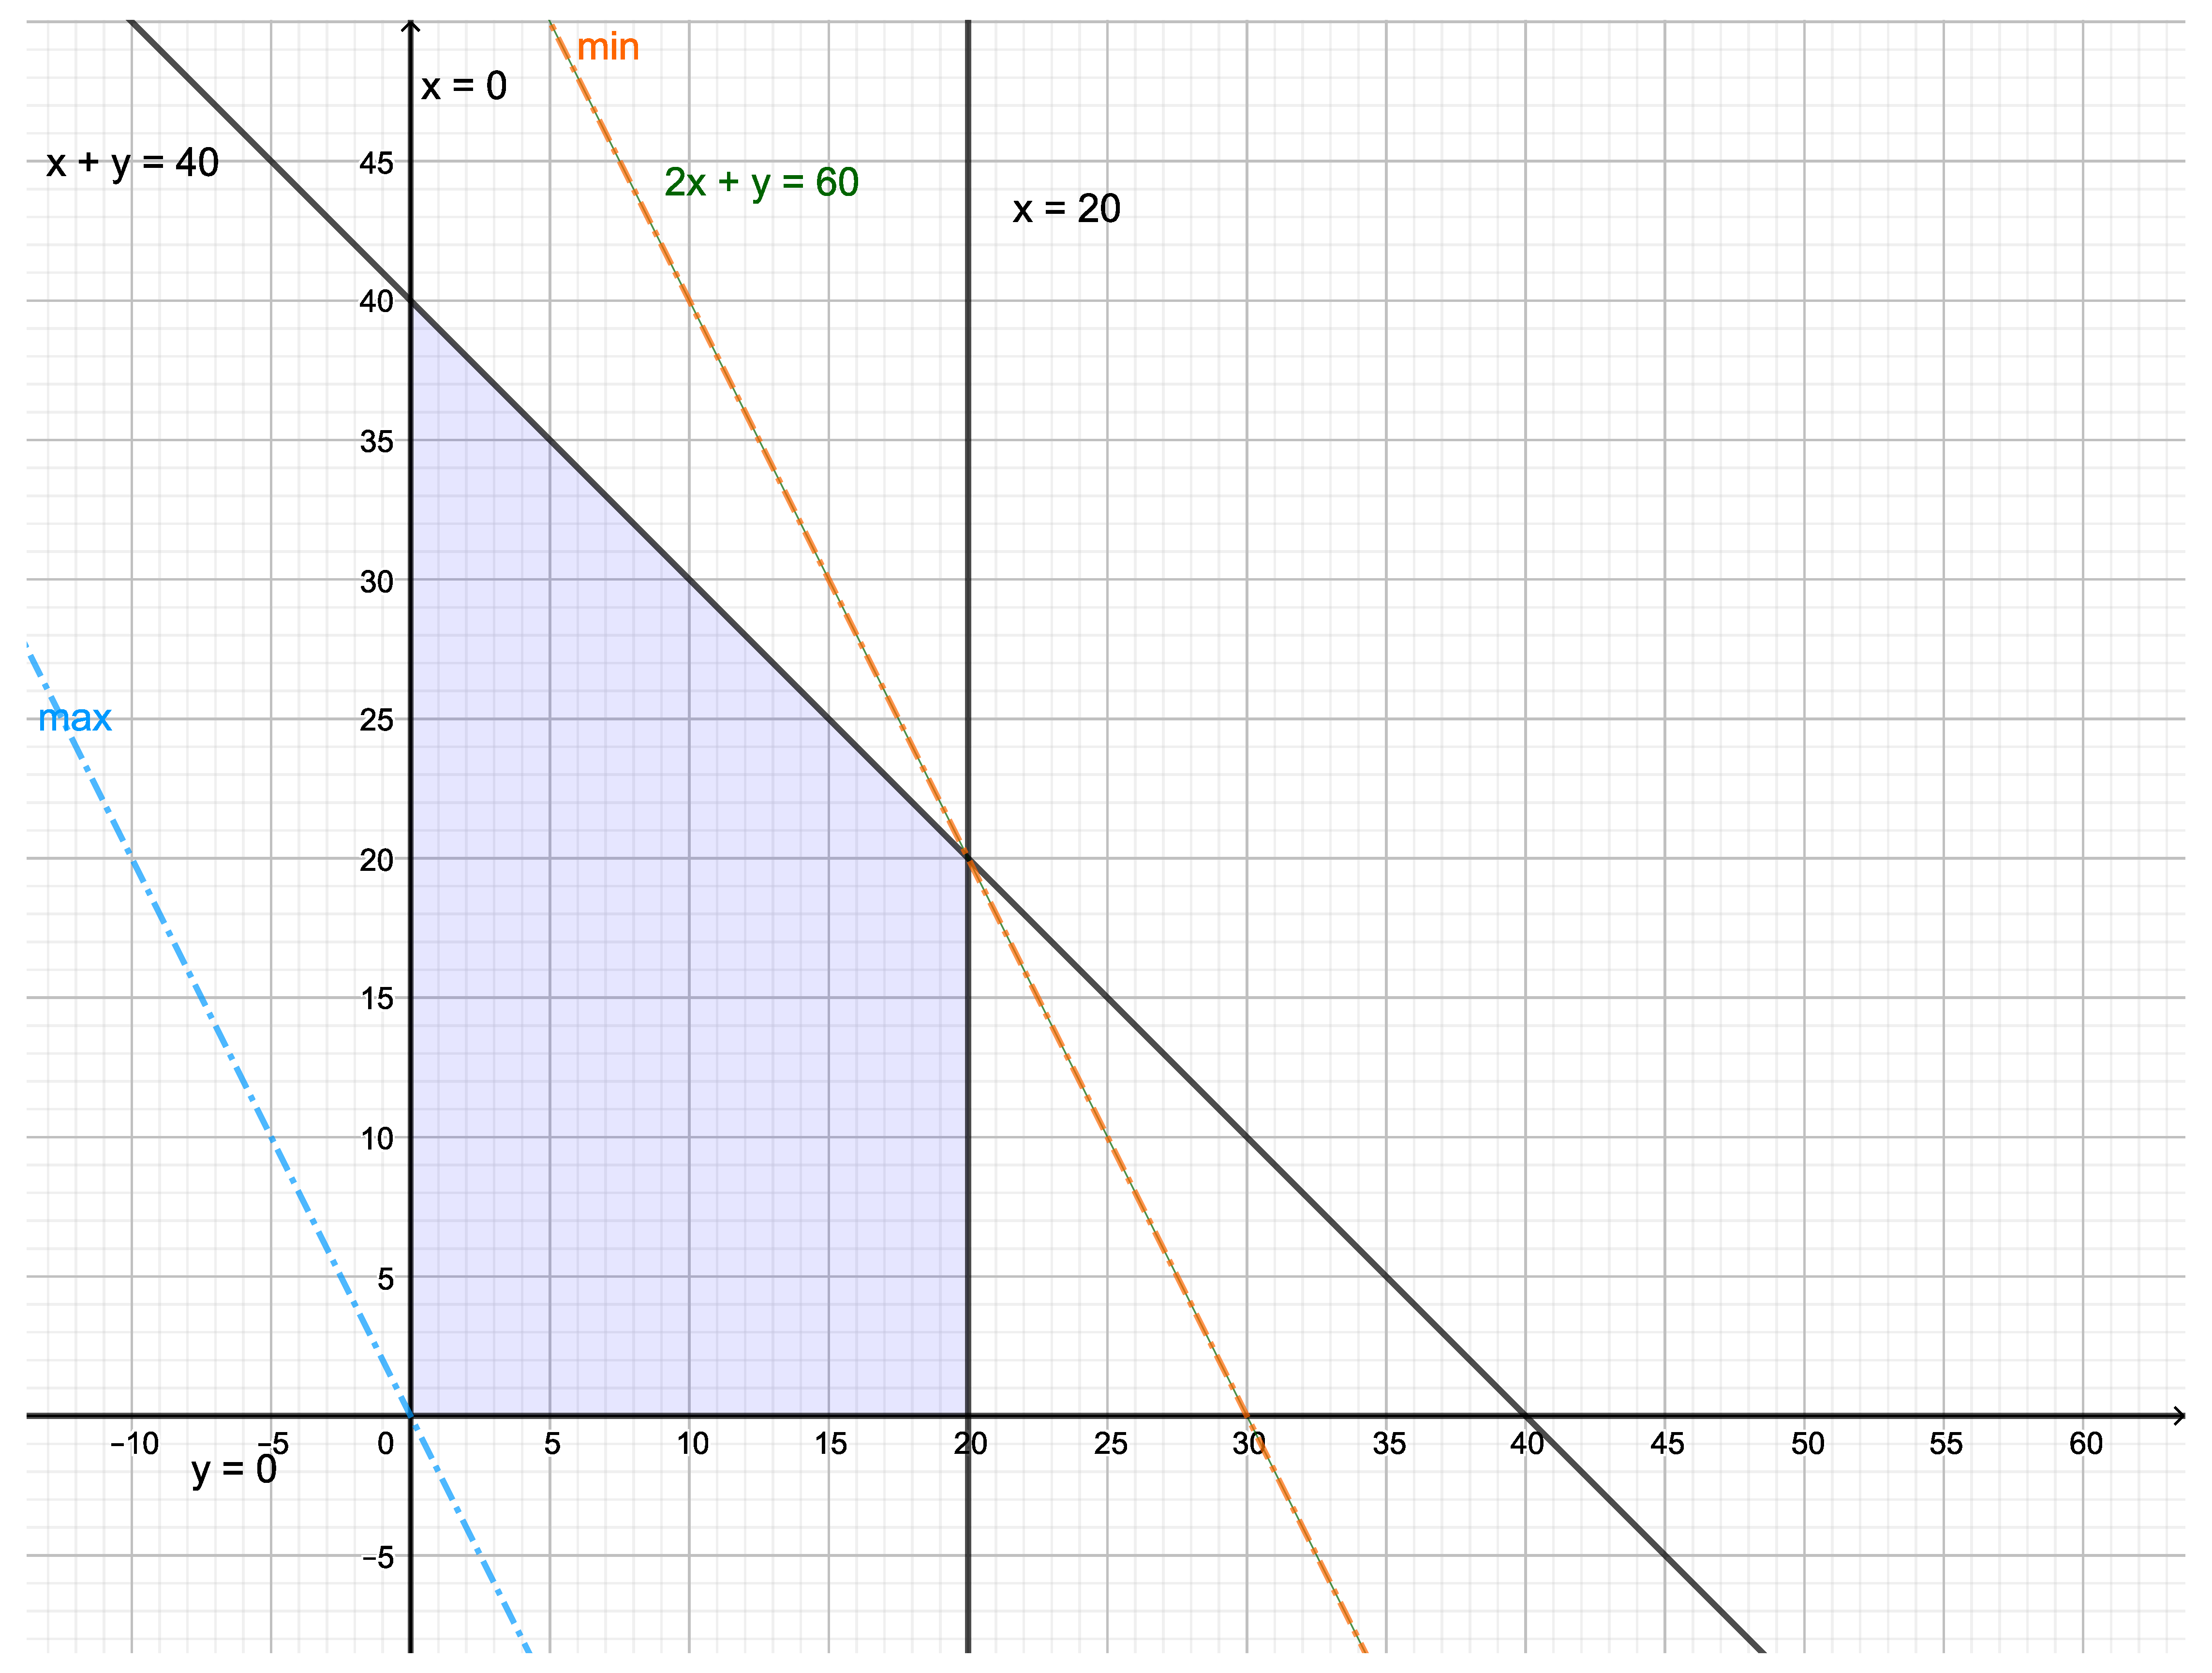
\includegraphics[width=0.5\textwidth]{2_8c.pdf}
\end{figure}
\begin{figure}[htbp]
  \caption{solution to (d)}
  \centering
    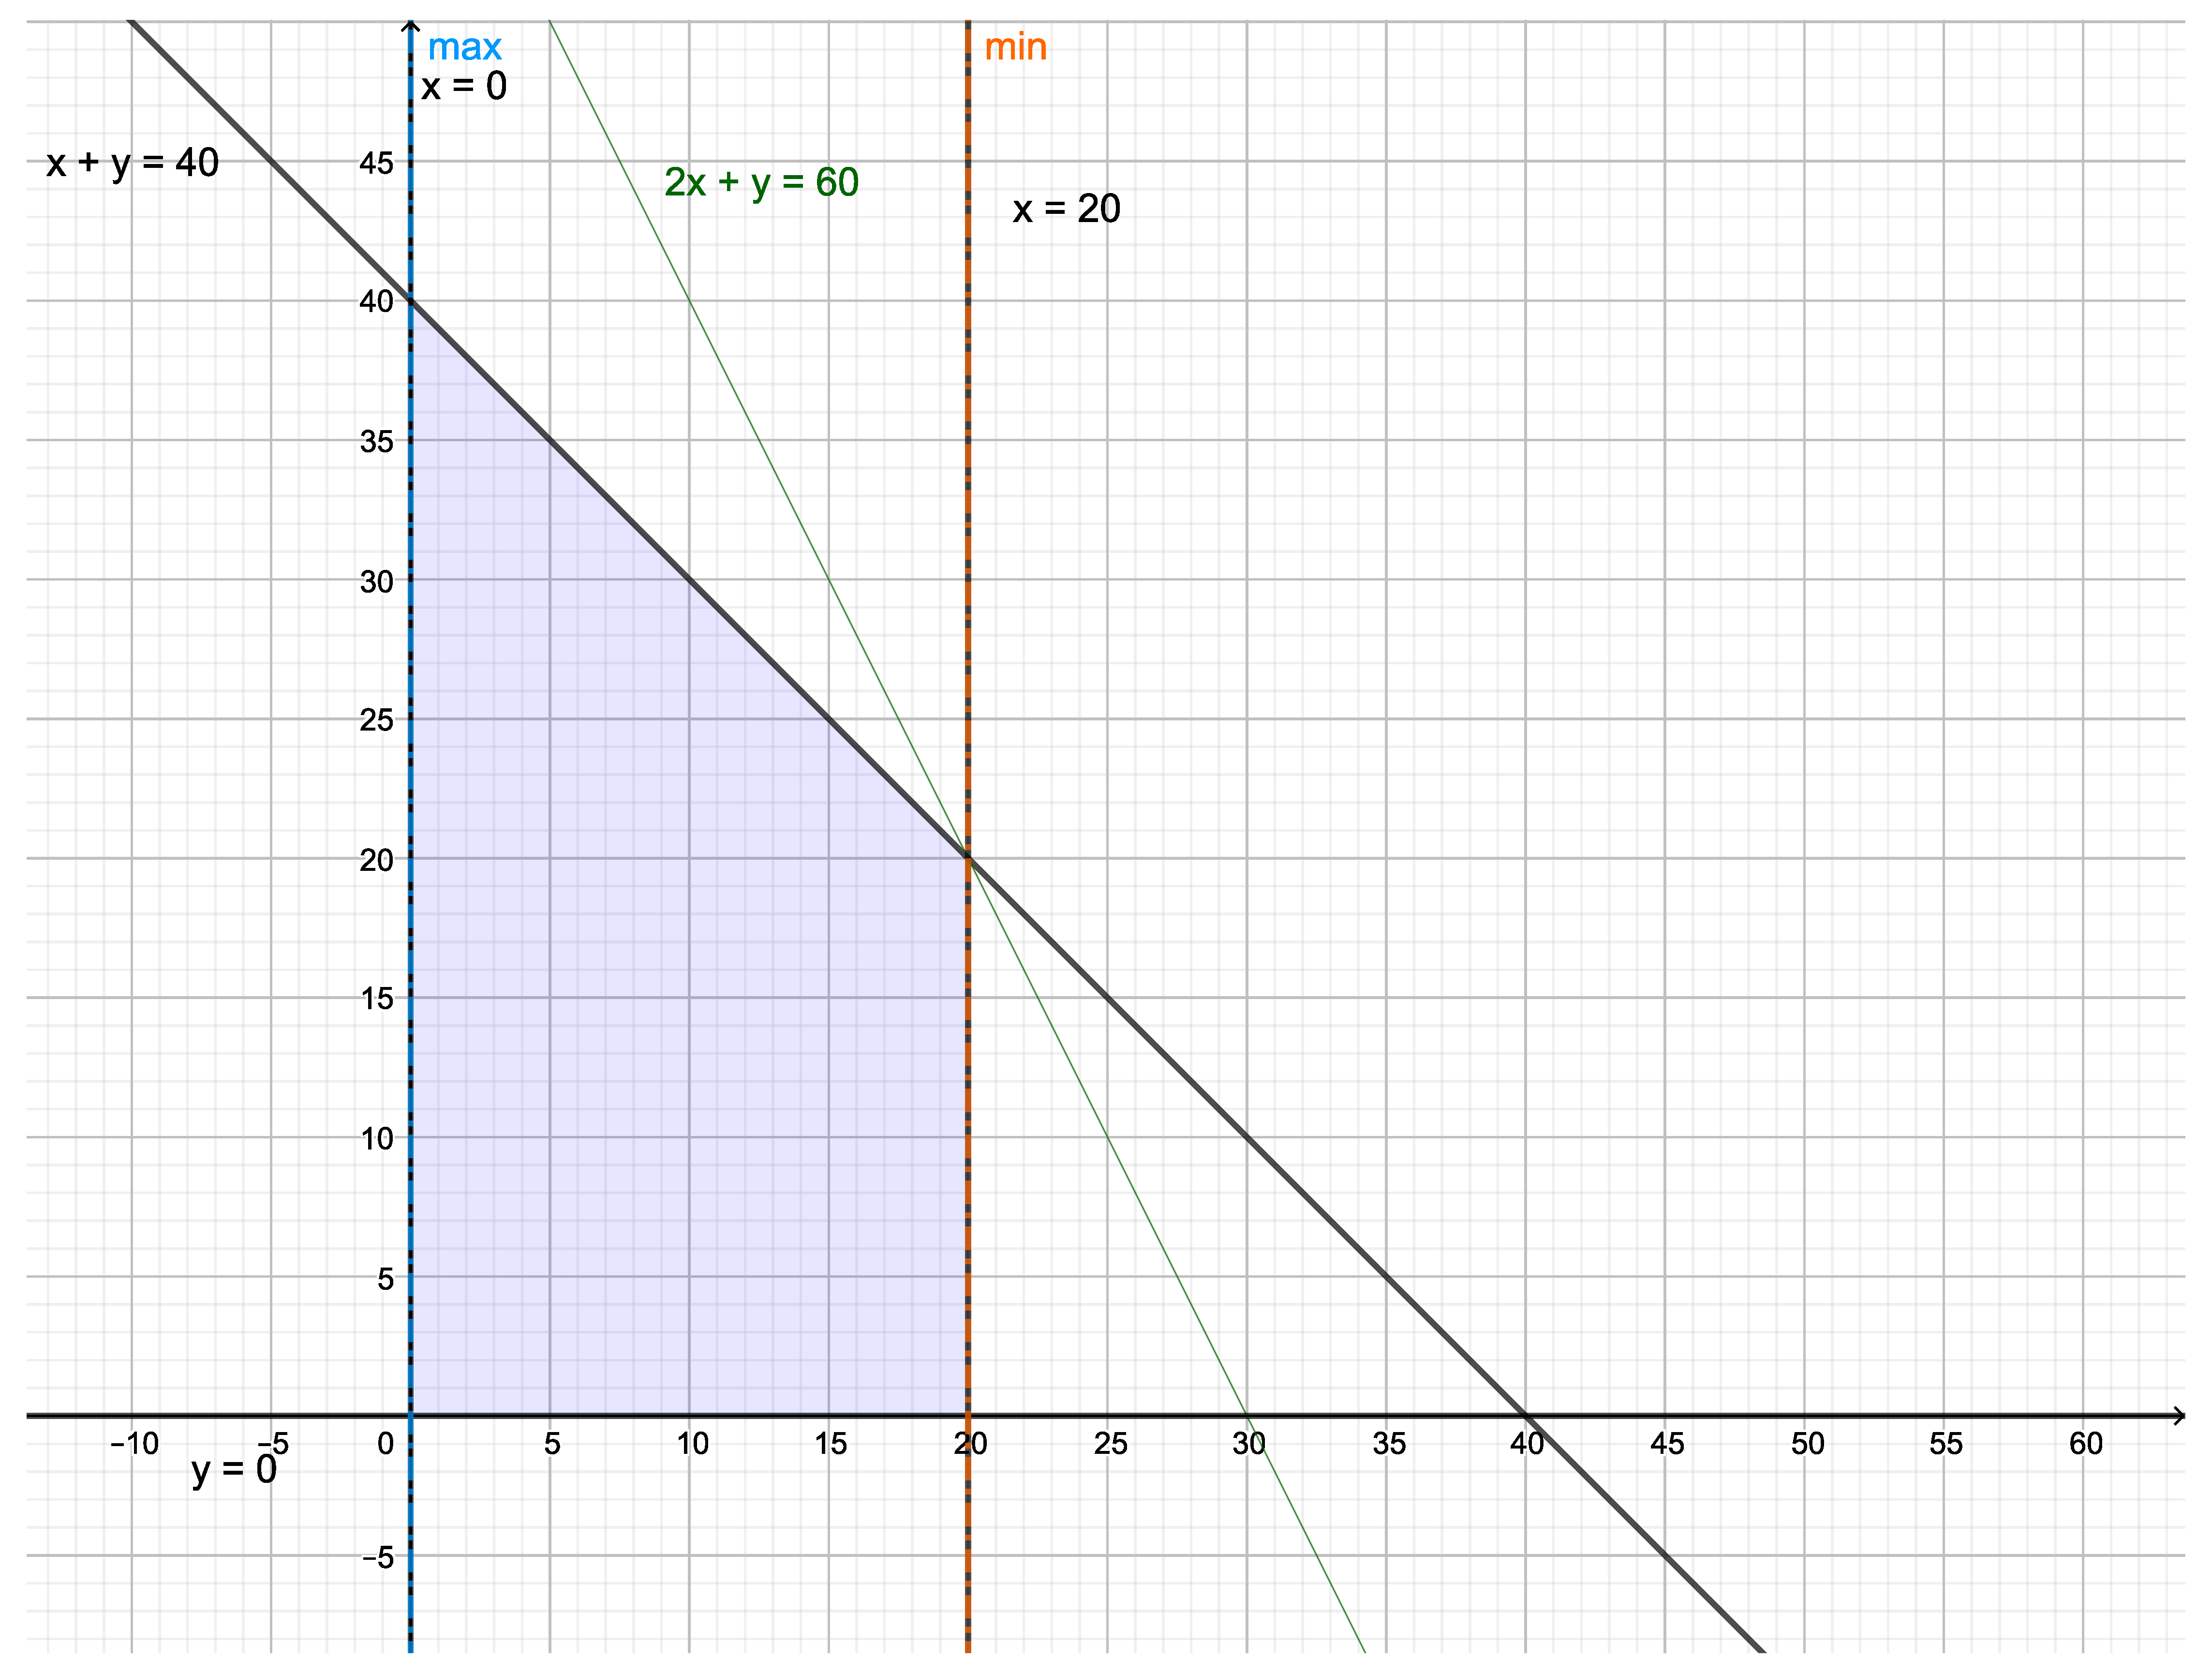
\includegraphics[width=0.5\textwidth]{2_8d.pdf}
\end{figure}
\begin{figure}[htbp]
  \caption{solution to (e)}
  \centering
    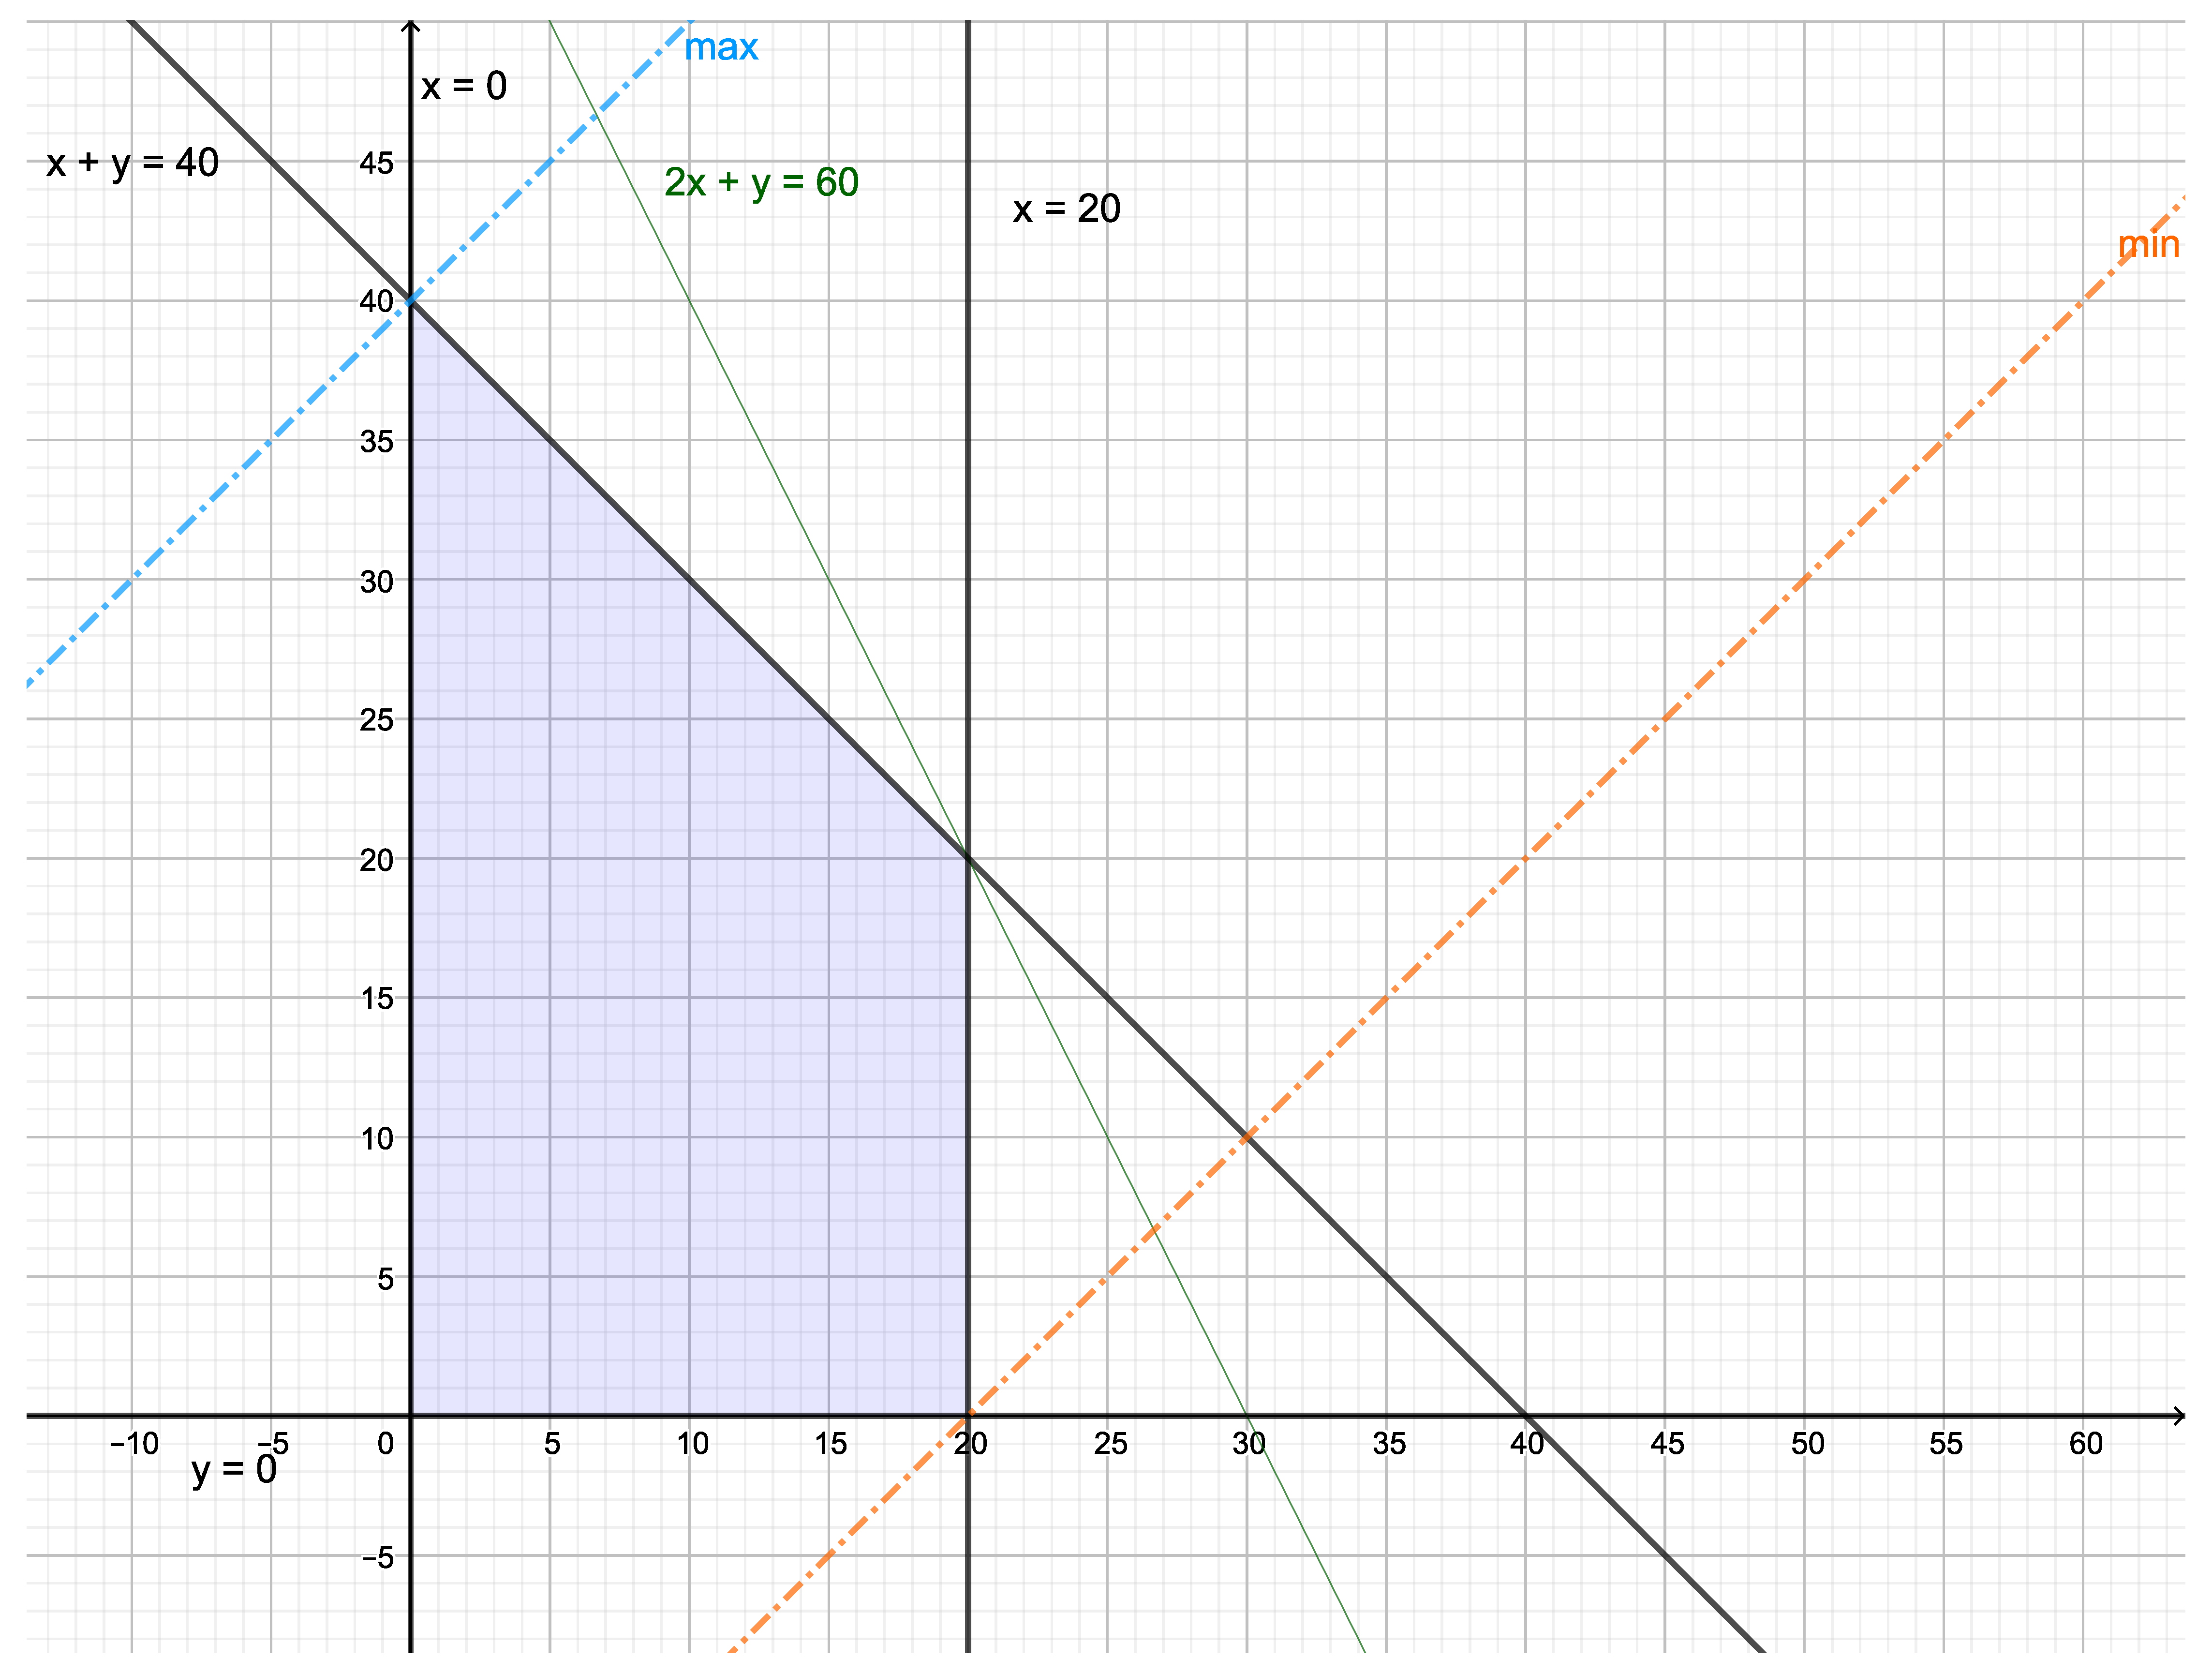
\includegraphics[width=0.5\textwidth]{2_8e.pdf}
\end{figure}

The optimal values can be tracked in the table.

\begin{table}
\centering
\caption{optimal solutions}
\label{2.8values}
\begin{tabular}{|c|c|c|}
\hline
  & max & min \\ \hline
a & 0   & -40 \\ \hline
b & 0   & -40 \\ \hline
c & 0   & -60 \\ \hline
d & 0   & -20 \\ \hline
e & 40  & -20 \\ \hline
\end{tabular}
\end{table}

\FloatBarrier

\section*{Problem 2.9}

\begin{proof}

Consider set $B$ as the set of optimal solutions to a Lp problem, which as the standard form,

\begin{equation*}
\begin{aligned}
\text{Minimize} \quad & c^Tx \\
\text{subject\  to} \quad & Ax = b \\
 & x \geqslant 0
\end{aligned}
\end{equation*}

where $A \in \mathbb{R}^{m\times n}$, $x\in \mathbb{R}^n$, $b \in \mathbb{R}^m$.

Denote its feasible domain as $P := \{x \in \mathbb{R}^n | Ax = b, x \geqslant 0 \}$. 

Suppose the optimal value is $M$, i.e., $\forall x^*, y^*\in B$, $c^Tx^* = x^Ty^* = M \leqslant c^Tx$, $\forall x\in P$.

Hence, take arbitrary $\alpha \in (0, 1)$, and it is true that $c^T(\alpha x^* + (1-\alpha) y^*) = M$. Hence, $B$ is convex.

\end{proof}

This result is useful to us. We know if there are two different optimal solutions to the LP problem, then any convex combination of those two solutions are also optimal.

\end{document}